% =========================================================================
% Capítulo 1: Cinemática
% Tema 03: Coordenadas intrínsecas
% Problema 01: Árbol de navidad
% =========================================================================
\subsubsection{Árbol de navidad}

Una partícula describe una trayectoria helicoidal cónica, donde el ángulo $\theta$
 representa la posición azimutal de la partícula y $r$ es la distancia radial entre la partícula 
 y el eje vertical. Además, $\beta$ es el ángulo formado entre el vector posición de la partícula 
 y el eje vertical (eje z).

\begin{figure}[!ht]
    \centering
    \begin{tikzpicture}[>=Latex, scale=1.5]
        
        % --- 1. EJES DE REFERENCIA ---
        \draw[->, gray!70] (0,0) -- (3,0) node[anchor=north east]{$x$};
        \draw[->, gray!70] (0,0) -- (0,4) node[anchor=south]{$z$};
        % Eje Y en perspectiva
        \draw[->, gray!70] (0,0) -- (-1.2,-1) node[anchor=north east]{$y$};

        % --- 2. PARÁMETROS DE LA ESPIRAL ---
        % Radio aumenta con la altura (z = k * r)
        % x = z * tan(beta) * cos(theta)
        % y = z * tan(beta) * sin(theta)
        \def\betaAng{30} % Ángulo del cono (beta)
        \def\k{0.57}      % tan(30°) aprox.
        
        % --- 3. LÍNEA GENERATRIZ DEL CONO ---
        \draw[thick] (0,0) -- ({3*\k}, 3.5) node[right, pos=0.8] {Generatriz};

        % --- 4. ESPIRAL CÓNICA (Trayectoria) ---
        % Dibujamos 4 vueltas (domain=0:8*pi)
        \draw[thick, blue!80!black] plot[domain=0:25, samples=200, variable=\t]
            ({0.1*\t * \k * cos(\t r) - 0.05*\t * \k * sin(\t r)}, 
             {0.13*\t}); 
             % Nota: El término negativo en x simula la inclinación del eje y

        % --- 5. PUNTO P ---
        % Elegimos un punto arbitrario en la espiral (t=14)
        \coordinate (P) at ({1.4 * \k * cos(14 r) - 0.7 * \k * sin(14 r)}, {1.4*1.3});
        \filldraw (P) circle (1.5pt) node[left, yshift=-4pt] {$P$};

        % --- 6. ÁNGULOS ---
        % Ángulo Beta (entre eje Z y generatriz)
        \draw[->, thick] (0,2) arc (90:65:2);
        \node at (0.35, 1.8) {$\beta$};

        % Ángulo Theta (azimutal en la base)
        % Dibujamos la proyección en el "suelo"
        \draw[dashed, gray] (0,0) -- (-0.85, -0.6);
        \draw[->, thick] (0.8, 0) arc (0:-125:0.8 and 0.4);
        \node at (-0.5, -0.8) {$\theta$};

    \end{tikzpicture}
    \caption{Trayectoria de una partícula $P$ que se desplaza sobre una superficie cónica. Se muestran las coordenadas angulares $\beta$ (polar) y $\theta$ (azimutal).}
    \label{fig:espiral_conica}
\end{figure}
 se conoce que $\dot{r}=c$ y $\theta= \dfrac{2\pi r}{R}$
\begin{enumerate}
    \item Defina marcos de referencia y sistemas de coordenadas.
    \item Determine la posición de $P$ según un observador fijo. 
    \item Determine la  velocidad y aceleración de $P$ según un observador fijo en el marco de referencia inercial. 
\end{enumerate}

% --- SOLUCIÓN ---------------------------------------------------------------
\begin{solucion}{Árbol de navidad}
\textbf{Defina marcos de referencia y sistemas de coordenadas.}
 \textbf{Respuesta:} Los marcos de referencia en este problema son:
    \begin{itemize}
        \item $\mathcal{N}$: Suelo (inercial).
        \item $\mathcal{A}$: Proyeccion del punto P sobre el plano XY con el centro.
    \end{itemize}
                Por otra parte, se definen los siguientes sistemas de coordenadas orto normales:
            \begin{itemize}
                \item $\{ \vec{e}_x, \vec{e}_y, \vec{e}_z \}$: Fijo en $\mathcal{N}$.
                \item $\{ \vec{e}_r, \vec{e}_{\theta}, \vec{e}_z \}$: Fijo en $\mathcal{A}$.
            \end{itemize}

\textbf{Determine la posición de $P$ según un observador fijo. }
\begin{center}
    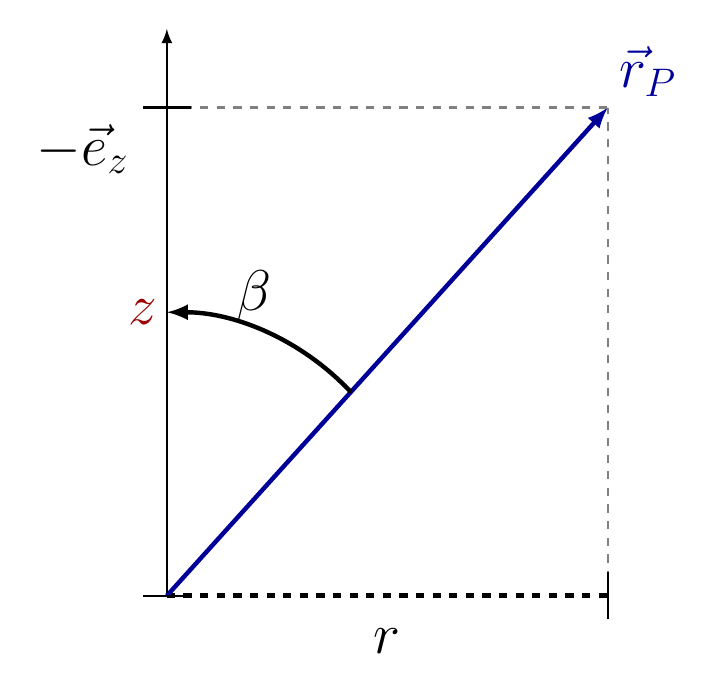
\begin{tikzpicture}
        % Vertical axis (solid) and horizontal axis (dashed)
        \draw[thick, -latex] (0, 0) -- (0, 7.2) node[anchor=north east, pos=0.85, xshift=-10pt] {\huge $-\vec{e}_z$};
        \draw[dashed, ultra thick] (0, 0) -- (5.6, 0);
        
        % Vector r_P
        \draw[ultra thick, blue!60!black, -latex] (0, 0) -- (5.6, 6.2) node[anchor=south west] {\huge $\vec{r}_P$};
        
        % Projected lines (dotted)
        \draw[dashed, thick, gray] (5.6, 0) -- (5.6, 6.2);
        \draw[dashed, thick, gray] (0, 6.2) -- (5.6, 6.2);
        
        % Labels
        \node[red!60!black, anchor=east] at (0, 3.6) {\huge $z$};
        \node[anchor=north] at (2.8, -0.3) {\huge $r$};
        
        % Ticks
        \draw[thick] (-0.3, 0) -- (0.3, 0);
        \draw[thick] (-0.3, 6.2) -- (0.3, 6.2);
        \draw[thick] (5.6, -0.3) -- (5.6, 0.3);
        
        % Angle arc
        \draw[ultra thick, black, latex-] (0, 3.6) arc [start angle=90, end angle=43, radius=3.2] node[midway, anchor=south, xshift=-5pt] {\huge $\beta$};
    \end{tikzpicture}
\end{center}
\textbf{Respuesta:} Notemos que, por geometría, la altura de la partícula está dada por
        \begin{equation}
            z = \frac{r}{\tan (\beta)}.
        \end{equation}
        
        Por lo tanto, la posición de la partícula puede describirse en coordenadas cilíndricas como
        \begin{align}
            \vec{r}_P &= r\vec{e}_{r} - z\vec{e}_z \\
                &= r\vec{e}_{r} - \frac{r}{\tan (\beta)} \vec{e}_z .
        \end{align}
Y de las relaciones se conoce que $\dot\theta=\dfrac{2\pi c}{R}$


       

\textbf{Determine la  velocidad y aceleración de $P$ según un observador fijo en el marco de referencia inercial.}



 Aplicando el Teorema de Transporte, la velocidad de $P$ nos queda:
        \begin{align*}
            \leftidx{^{\mathcal{N}}}{\vec{v}}{_P} = \leftidx{^{\mathcal{N}}}{\frac{d}{dt}}{} \left( \vec{r}_P \right) &=  \leftidx{^{\mathcal{A}}}{\frac{d}{dt}}{} \left( \vec{r}_P \right) + \leftidx{^{\mathcal{N}}}{\vec{\omega}}{^{\mathcal{A}}} \times \vec{r}_P \\
                &= \dot{r}\vec{e}_{r} - \frac{\dot{r}}{\tan (\beta)} \vec{e}_z + \dot{\theta} \vec{e}_z \times \left( r\vec{e}_{r} - \frac{r}{\tan (\beta)} \vec{e}_z \right) \\
                &= \dot{r}\vec{e}_{r} + r\dot{\theta} \vec{e}_{\theta} - \frac{\dot{r}}{\tan (\beta)} \vec{e}_z .\\
                &= c\vec{e}_{r} + r\dfrac{2\pi c}{R} \vec{e}_{\theta} - \frac{c}{\tan (\beta)} \vec{e}_z .
        \end{align*}

        Para obtener la aceleración podemos aplicar nuevamente Teorema de Transporte:
        \begin{align}
            \leftidx{^{\mathcal{N}}}{\vec{a}}{_P} = \leftidx{^{\mathcal{N}}}{\frac{d}{dt}}{} \left( \leftidx{^{\mathcal{N}}}{\vec{v}}{_P} \right) &= \leftidx{^{\mathcal{A}}}{\frac{d}{dt}}{} \left( \leftidx{^{\mathcal{N}}}{\vec{v}}{_P} \right) + \leftidx{^{\mathcal{N}}}{\vec{\omega}}{^{\mathcal{A}}} \times \leftidx{^{\mathcal{N}}}{\vec{v}}{_P} \\
                &= \ddot{r}\vec{e}_{r} + \left( \dot{r}\dot{\theta} + r\ddot{\theta} \right) \vec{e}_{\theta} - \frac{\ddot{r}}{\tan (\beta)} \vec{e}_z + \dot{\theta} \vec{e}_z \times \left( \dot{r}\vec{e}_{r} + r\dot{\theta} \vec{e}_{\theta} - \frac{\dot{r}}{\tan (\beta)} \vec{e}_z \right) \\
                &= \ddot{r}\vec{e}_{r} + \left( \dot{r}\dot{\theta} + r\ddot{\theta} \right) \vec{e}_{\theta} - \frac{\ddot{r}}{\tan (\beta)} \vec{e}_z + \dot{r}\dot{\theta}\vec{e}_{\theta} - r\dot{\theta}^2 \vec{e}_{r} \\
                &= \left( \ddot{r} - r\dot{\theta}^2 \right) \vec{e}_r + \left( 2\dot{r}\dot{\theta} + r\ddot{\theta} \right) \vec{e}_{\theta} - \frac{\ddot{r}}{\tan (\beta)} \vec{e}_z .
        \end{align}
        A su vez se conoce que $\dot{r}=c$ por ende $\ddot{r}=0$ y que $\dot\theta=\dfrac{2\pi c}{R}$ asi mismo  $\ddot\theta=0$

                \begin{equation}
             \leftidx{^{\mathcal{N}}}{\vec{a}}{_P}=\left(-r\left(\dfrac{2\pi c}{R}\right)^2\right)\vec{e}_r+\left(2c\dfrac{2\pi c}{R}\right)\vec{e}_{\theta}
        \end{equation}
\end{solucion}


% --- SOLUCIÓN ---------------------------------------------------------------
\begin{solucion}{Árbol de navidad (sin condición sobre $R$ y $\theta$)}
\vspace{0.8em}
\noindent\textbf{1. Definición de marcos de referencia y sistemas de coordenadas}

Para abordar el problema, identificamos los siguientes marcos de referencia:
\begin{itemize}
    \item $\mathcal{N}$: Marco de referencia inercial asociado al suelo.
    \item $\mathcal{A}$: Marco de referencia no inercial (imaginario) que gira de manera solidaria con el incremento del ángulo azimutal $\theta$.
\end{itemize}

Asimismo, definimos dos sistemas de coordenadas ortonormales para describir el movimiento:
\begin{itemize}
    \item $\{ \vec{e}_x, \vec{e}_y, \vec{e}_z \}$: Sistema fijo en el marco inercial $\mathcal{N}$.
    \item $\{ \vec{e}_r, \vec{e}_{\theta}, \vec{e}_z \}$: Sistema cilíndrico fijo en el marco móvil $\mathcal{A}$.
\end{itemize}

\vspace{0.8em}
\noindent\textbf{2. Posición, velocidad y aceleración de la partícula}

\textbf{pregunta sin puntaje} Determine la posición, velocidad y aceleración de $P$ según un observador fijo en el marco de referencia inercial.

\paragraph{Posición:} A partir de la geometría del cono, la altura $z$ de la partícula se relaciona con el radio $r$ mediante la constante $\beta$:
\[
    z = \frac{r}{\tan(\beta)}.
\]
De este modo, expresamos el vector de posición de $P$ en coordenadas cilíndricas como:
\begin{align*}
    \vec{r}_P &= r\vec{e}_{r} - z\vec{e}_z \\
              &= r\vec{e}_{r} - \frac{r}{\tan(\beta)} \vec{e}_z.
\end{align*}

\paragraph{Velocidad:} Para calcular la velocidad desde el marco inercial $\mathcal{N}$, derivamos la posición empleando el Teorema de Transporte:
\begin{align*}
    \leftidx{^{\mathcal{N}}}{\vec{v}}{_P} &= \leftidx{^{\mathcal{N}}}{\frac{d}{dt}}{} \left( \vec{r}_P \right) = \leftidx{^{\mathcal{A}}}{\frac{d}{dt}}{} \left( \vec{r}_P \right) + \leftidx{^{\mathcal{N}}}{\vec{\omega}}{^{\mathcal{A}}} \times \vec{r}_P \\
    &= \left( \dot{r}\vec{e}_{r} - \frac{\dot{r}}{\tan(\beta)} \vec{e}_z \right) + \left( \dot{\theta} \vec{e}_z \right) \times \left( r\vec{e}_{r} - \frac{r}{\tan(\beta)} \vec{e}_z \right) \\
    &= \dot{r}\vec{e}_{r} + r\dot{\theta} \vec{e}_{\theta} - \frac{\dot{r}}{\tan(\beta)} \vec{e}_z.
\end{align*}

\paragraph{Aceleración:} Aplicamos nuevamente el Teorema de Transporte sobre el vector velocidad:
\begin{align*}
    \leftidx{^{\mathcal{N}}}{\vec{a}}{_P} &= \leftidx{^{\mathcal{N}}}{\frac{d}{dt}}{} \left( \leftidx{^{\mathcal{N}}}{\vec{v}}{_P} \right) = \leftidx{^{\mathcal{A}}}{\frac{d}{dt}}{} \left( \leftidx{^{\mathcal{N}}}{\vec{v}}{_P} \right) + \leftidx{^{\mathcal{N}}}{\vec{\omega}}{^{\mathcal{A}}} \times \leftidx{^{\mathcal{N}}}{\vec{v}}{_P} \\
    &= \left( \ddot{r}\vec{e}_{r} + (\dot{r}\dot{\theta} + r\ddot{\theta})\vec{e}_{\theta} - \frac{\ddot{r}}{\tan(\beta)}\vec{e}_z \right) + \dot{\theta}\vec{e}_z \times \left( \dot{r}\vec{e}_{r} + r\dot{\theta}\vec{e}_{\theta} - \frac{\dot{r}}{\tan(\beta)}\vec{e}_z \right) \\
    &= \left( \ddot{r} - r\dot{\theta}^2 \right)\vec{e}_r + \left( 2\dot{r}\dot{\theta} + r\ddot{\theta} \right)\vec{e}_{\theta} - \frac{\ddot{r}}{\tan(\beta)}\vec{e}_z.
\end{align*}
Dado que la rapidez radial es constante ($\dot{r} = c$), su derivada temporal es nula ($\ddot{r} = 0$). Sustituyendo esta condición, la aceleración simplificada resulta:
\[
    \leftidx{^{\mathcal{N}}}{\vec{a}}{_P} = (-r\dot{\theta}^2)\vec{e}_r + (2c\dot{\theta} + r\ddot{\theta})\vec{e}_{\theta}.
\]

\vspace{0.8em}
\noindent\textbf{3. Distancia radial en el punto $Q$ donde la rapidez es $3c$}

Primero, determinamos la norma del vector velocidad en cualquier instante:
\begin{align*}
    \leftidx{^{\mathcal{N}}}{v}{_P} := \| \leftidx{^{\mathcal{N}}}{\vec{v}}{_P} \| &= \sqrt{ \dot{r}^2 + r^2\dot{\theta}^2 + \left( -\frac{\dot{r}}{\tan(\beta)} \right)^2 }.
\end{align*}
Evaluando la condición $\leftidx{^{\mathcal{N}}}{v}{_P} = 3c$ para el punto $Q$ (usando $\dot{r} = c$):
\begin{align*}
    \sqrt{ c^2 + r^2\dot{\theta}^2 + \left( \frac{c}{\tan(\beta)} \right)^2 } &= 3c \\
    \Leftrightarrow c^2 + r^2\dot{\theta}^2 + \frac{c^2}{\tan^2(\beta)} &= 9c^2 \\
    \Leftrightarrow r^2\dot{\theta}^2 &= c^2 \left( 8 - \frac{1}{\tan^2(\beta)} \right).
\end{align*}
Despejando el radio $r$, encontramos la distancia radial en $Q$:
\begin{align*}
    r = \frac{c}{\dot{\theta}} \sqrt{8 - \frac{1}{\tan^2(\beta)}}.
\end{align*}

\vspace{0.8em}
\noindent\textbf{4. Radio de curvatura en el punto $Q$}



El radio de curvatura $R$ se define conceptualmente a través de la rapidez y la magnitud de la derivada del vector unitario tangente $\vec{e}_t$:
\[
    R = \frac{1}{\kappa} = \frac{\leftidx{^{\mathcal{N}}}{v}{_P}}{\left\| \leftidx{^{\mathcal{N}}}{\frac{d}{dt}}{} (\vec{e}_t) \right\|}.
\]
Construimos el vector tangente unitario usando la relación $\cot(\beta) = \frac{1}{\tan(\beta)}$:
\begin{align*}
    \vec{e}_t = \frac{c\vec{e}_r + r\dot{\theta}\vec{e}_{\theta} - c\cot(\beta)\vec{e}_z}{\sqrt{c^2(1+\cot^2(\beta)) + (r\dot{\theta})^2}}.
\end{align*}
Derivamos el vector $\vec{e}_t$ con respecto al tiempo dividiendo el proceso por la regla del producto:
\begin{align*}
    \leftidx{^{\mathcal{N}}}{\frac{d}{dt}}{} \left( c\vec{e}_r + r\dot{\theta}\vec{e}_\theta - c\cot(\beta)\vec{e}_z \right) &= -r\dot{\theta}^2\vec{e}_r + (2c\dot{\theta} + r\ddot{\theta})\vec{e}_{\theta}, \\
    \leftidx{^{\mathcal{N}}}{\frac{d}{dt}}{} \left( \frac{1}{\sqrt{c^2(1+\cot^2(\beta)) + (r\dot{\theta})^2}} \right) &= -\frac{r\dot{\theta}(r\ddot{\theta} + c\dot{\theta})}{\left(c^2(\cot^2(\beta)+1) + (r\dot{\theta})^2\right)^{3/2}}.
\end{align*}

Evaluando la norma del denominador en el punto $Q$ (donde la norma de la velocidad vale $3c$):
\[
    \sqrt{c^2(1+\cot^2(\beta)) + (r\dot{\theta})^2} = 3c.
\]
Sustituyendo y agrupando componentes en $\vec{e}_r$, $\vec{e}_\theta$ y $\vec{e}_z$:
\begin{align*}
    \left\| \leftidx{^{\mathcal{N}}}{\frac{d}{dt}}{} (\vec{e}_t) \right\| &= \frac{1}{(3c)^3} \left\| -(r\dot{\theta}^2(3c)^2 + c r\dot{\theta}(r\ddot{\theta}+c\dot{\theta}))\vec{e}_r + ((2c\dot{\theta}+r\ddot{\theta})(3c)^2 - (r\dot{\theta})^2(r\ddot{\theta}+c\dot{\theta}))\vec{e}_{\theta} + c\cot(\beta)r\dot{\theta}(r\ddot{\theta}+c\dot{\theta})\vec{e}_z \right\| \\
    &= \frac{1}{(3c)^3} \sqrt{ (r\dot{\theta})^2 \left( (\dot{\theta}(3c)^2 + c(r\ddot{\theta}+c\dot{\theta}))^2 + (c\cot(\beta)(r\ddot{\theta}+c\dot{\theta}))^2 \right) + \left( (2c\dot{\theta}+r\ddot{\theta})(3c)^2 - (r\dot{\theta})^2(r\ddot{\theta}+c\dot{\theta}) \right)^2 }.
\end{align*}
Finalmente, utilizando $v_P = 3c$, el radio de curvatura en $Q$ resulta:
\[
    R = \frac{(3c) \cdot (3c)^3}{\sqrt{ (r\dot{\theta})^2 \left( (\dot{\theta}(3c)^2 + c(r\ddot{\theta}+c\dot{\theta}))^2 + (c\cot(\beta)(r\ddot{\theta}+c\dot{\theta}))^2 \right) + \left( (2c\dot{\theta}+r\ddot{\theta})(3c)^2 - (r\dot{\theta})^2(r\ddot{\theta}+c\dot{\theta}) \right)^2 }}.
\]

\vspace{0.8em}
\noindent\textbf{5. Longitud de arco recorrida hasta el punto $Q$}

\textbf{pregunta sin puntaje} Encuentre una expresión para la longitud de arco recorrida por la partícula desde que parte en el vértice de la espiral hasta que alcanza el punto $Q$.

Por definición, la longitud de arco recorrida $s(t^*)$ desde el reposo/vértice ($t_0 = 0$, $s(0) = 0$) corresponde a la integral temporal de la rapidez:
\[
    s(t^*) = \int_{0}^{t^*} \leftidx{^{\mathcal{N}}}{v}{_P} \, dt = \int_{0}^{t^*} \sqrt{ c^2 + (ct)^2\dot{\theta}^2 + \left( -\frac{c}{\tan(\beta)} \right)^2 } \, dt,
\]
donde hemos utilizado $r(t) = c \cdot t$.

Para determinar el límite superior de integración $t^*$, tomamos la relación obtenida en el punto $Q$:
\[
    r\dot{\theta} = c \sqrt{8 - \frac{1}{\tan^2(\beta)}} \implies t^* \dot{\theta} = \sqrt{8 - \frac{1}{\tan^2(\beta)}}.
\]
Definiendo una función auxiliar $g(t) = t \cdot \dot{\theta}(t)$, podemos despejar el tiempo $t^*$ mediante su función inversa:
\[
    t^* = g^{-1}\left( \sqrt{8 - \frac{1}{\tan^2(\beta)}} \right).
\]
Sustituyendo el límite de integración, la expresión final para la longitud de arco es:
\[
    s(t^*) = \int_{0}^{g^{-1}\left( \sqrt{8 - \frac{1}{\tan^2(\beta)}} \right)} \sqrt{ c^2 + (ct)^2\dot{\theta}^2 + \left( -\frac{c}{\tan(\beta)} \right)^2 } \, dt.
\]
\end{solucion}

